\begin{problem}{\textbf{\textsc{Devil's Trill}}}
Consider a string of length $L=1\;\mathrm{m}$ and linear mass density $\lambda$\ =\ 1\ g/m, fixed on both ends and vibrating in the first normal mode with amplitude $A = 0.125 \; \mathrm{cm}$. A frictionless, negligibly-small finger, initially at the right endpoint, slides slowly toward the left, flattening the oscillation as it goes. When the vibrating part of the string has length $L_2=12.5\;\mathrm{cm}$, find the new amplitude of vibrations $A_2$, in meters. You may assume $A_2\ll L_2$. Diagrams are not necessarily drawn to scale. 

\FloatBarrier
\begin{figure*}[!htbp]
\centering
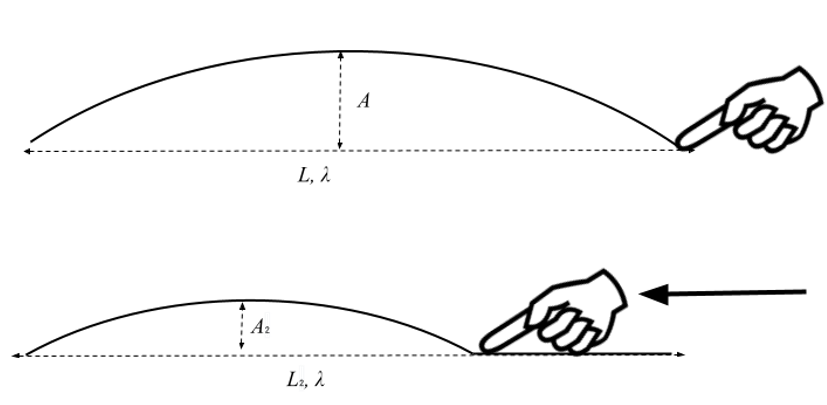
\includegraphics[width=0.6\textwidth]{problems/figures/devilTrill.png}
\end{figure*}
\FloatBarrier



\end{problem}